\section{Pattern detection}
\label{sec:pd}


% ----------------------- paths to graphics ------------------------



% ----------------------- contents from here ------------------------
% 

We use the term \textit{pattern detection} to refer to the process of identifying patterns in the data and evaluating its \textit{whitebox} representation potential. We introduce the concept of \textit{pattern detector}---a modular component in a generic compression learning architecture. This section presents the generic interface of a pattern detector and 5 specialized implementations of it.

\subsection{Generic pattern detector}
\label{subsec:genericpd}


% ----------------------- paths to graphics ------------------------



% ----------------------- contents from here ------------------------
% 

The purpose of a generic pattern detector is to serve as an interface in the pattern detection and compression learning processes. Given a sample of data and its schema, an instance of a generic pattern detector searches for the presence of the pattern it is specialized in.  For each column that matches the pattern, it outputs metrics and metadata that will be further used in the learning phase and during compression. This generic design allows new pattern detectors to be easily tested and integrated into the system without modifying other parts of it (e.g. the learning or compression processes). This section presents the characteristics of the generic pattern detector interface, while specialized implementations of it are described in the next sections.

The pattern detection process works in 3 phases: Phase-1: \textit{initialization}---initializes the pattern detector and creates the data structures that will be used in the next phases; Phase-2: \textit{scanning}---scans the sample of data and gathers information and metrics about values in the sample. Phase-3: \textit{evaluation}---aggregates the information gathered in the \textit{scanning} phase and produces an evaluation result.

\textbf{Parameters.} A pattern detector takes as input the following parameters:\\
a) \textit{columns}: id, name and datatype for each column\\
b) \textit{compression tree}: the compression tree built so far. Used in the \textit{select\_column} method\\
c) \textit{detection log}: history of the pattern detection process. Contains information about which pattern detectors were evaluated on each column and what was the result. Used in the \textit{select\_column} method.\\
Although most pattern detectors work on individual columns, some may work on multiple columns (e.g. \nameref{subsec:pd:columncorrelation}). For this reason we designed the generic pattern detector to search for patterns at the table level instead of individual columns.

\textbf{Methods.} A pattern detector must implement the following methods:\\
a) \textit{select\_column}: called in the \textit{initialization} phase---determines whether a given column will be processed by the pattern detector. The decision process is based on: 1) data type (e.g. string-specific patterns do not apply to numeric columns); 2) path in the compression tree that led to the creation of the column (e.g. \nameref{subsec:pd:columncorrelation} only applies to columns that are output of a \nameref{subsec:pd:dict} compression node); 3) history of the pattern detection process (e.g. do not evaluate a pattern detector on a column if it was already evaluated in a previous step). Column selection rules are listed in the section of each pattern detector.\\
b) \textit{feed\_tuple}: repeatedly called in the \textit{scanning} phase---processes a tuple. Data is fed to the pattern detector one tuple at a time. This method extracts information from the tuple that will be later used in the \textit{evaluate} method.\\
c) \textit{evaluate}: called in the \textit{evaluation} phase---aggregates the information extracted from the tuples fed so far and outputs the outcome of applying the pattern to the columns. See output details below.

\textbf{Output.} The result of evaluating a pattern detector on a sample of data is a list of \textit{(expression node, evaluation result)} tuples.\\
a) \textit{expression node}: describes how one or more \textit{input columns} are transformed into one or more \textit{output columns} by applying an \textit{operator} (see detailed description in \ref{ch:exprlang}~\nameref{ch:exprlang}). An important part here is the operator metadata that will be used to evaluate the \textit{expression node} in the (de)compression process (e.g. the operator metadata for the \nameref{subsec:pd:dict} pattern detector is the dictionary/map object).\\
b) \textit{evaluation result}: contains information used in the learning process and describes how well the \textit{input columns} of the \textit{expression node} match the pattern. It contains the following information: 1) \textit{coverage} (percentage of rows that the pattern applies to; i.e. \(1 - exception\_ratio\)); 2) \textit{row\_mask} (bitmap indicating the rows that the pattern applies to); 3) other pattern-specific evaluation results (e.g. correlation coefficient for column correlation).

Each \textit{(expression node, evaluation result)} tuple represents a possibility of applying the pattern on a subset of the columns. The same column may be present in multiple tuples since there may be more than one option of applying the pattern to it (e.g. the \nameref{subsec:pd:charsetsplit} pattern detector can split a column in 2 ways, because there are 2 dominant character set patterns on the column; see \ref{subsec:pd:charsetsplit}~\nameref{subsec:pd:charsetsplit} for more details). The \textit{row\_masks} for such a column may either be mutually exclusive or partially overlap. A pattern detector only outputs results for columns that match the pattern and are likely to produce good results in the compression process according to a pattern-specific estimator (e.g. \nameref{subsec:pd:dict} pattern detector only outputs tuples for columns that are dictionary compressible; see \ref{subsec:pd:dict}~\nameref{subsec:pd:dict} for more details).

\textbf{Operators.} Each pattern detector provides a \textit{compression operator} and a \textit{decompression operator}. They are used in the compression and respectively decompression phase to evaluate the nodes in the expression trees. The generic operator is described in \ref{ch:exprlang}~\nameref{ch:exprlang} while the pattern-specific implementations can be found in the corresponding section of each pattern detector.

% TODO-1: image describing the input and output of the generic pattern detector

% ---------------------------------------------------------------------------
% ----------------------- end of thesis sub-document ------------------------
% ---------------------------------------------------------------------------

\subsection{Constant}
\label{subsec:pd:constant}


% ----------------------- paths to graphics ------------------------

\graphicspath{{5_automatic_learning/pattern_detection/images/}}

% ----------------------- contents from here ------------------------
% 

The \nameref{subsec:pd:constant} pattern detector identifies columns that have (mostly) a single value. We refer to these columns as being constant. An additional parameter is provided in the initialization: \(constant\_ratio_{min}\) which indicates the minimum ratio of the constant value, based on which a column is considered constant or not. This pattern detector works on all data types, therefore the \textit{select\_column} method always returns \textit{True}. This is a single-column pattern detector and columns are evaluated independently. The next paragraphs describe the pattern detection process for a single column.

The \textit{scanning} phase is responsible for building the histogram of values on the column. The \textit{evaluation} phase selects the most common value \(C\) as the constant candidate---the value with the highest number of occurrences. The \(constant\_ratio\) of the column represents the evaluation metric and is computed as follows:
\begin{equation}
\label{eq:pd:constant:constantratio}
    constant\_ratio = \frac{count_{C}}{count_{notnull}}
\end{equation}
where:
\begin{itemize}
    \item[] \(count_{C}\) = number of occurrences of the constant candidate \(C\)
    \item[] \(count_{notnull}\) = number of non-null values in the column
\end{itemize}

The column is considered to fit the \nameref{subsec:pd:constant} pattern if the \(constant\_ratio\) is greater or equal to \(constant\_ratio_{min}\). All values that are not equal to \(C\) are considered exceptions. The \textit{evaluation result} is composed of the \textit{coverage} and \textit{row\_mask}---as defined in \ref{subsec:genericpd}~\nameref{subsec:genericpd}---and the \(constant\_ratio\) as an additional pattern-specific result. The metadata needed for compression and decompression is the constant \(C\).

The \textit{expression nodes} for the \nameref{subsec:pd:constant} pattern are illustrated in Figure~\ref{fig:pd:constant:exprnode}.

\begin{figure}[h]
  \centering
  \begin{subfigure}[t]{0.4\linewidth}
    \centering
    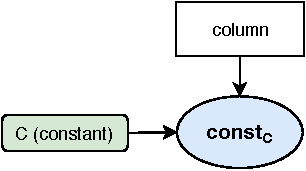
\includegraphics[width=0.8\linewidth]{expression_node-constant-compression_2.pdf}
    \caption[b]{compression}
    \label{fig:pd:constant:exprnode:compression}
  \end{subfigure}
  \hspace{1em}
  \begin{subfigure}[t]{0.4\linewidth}
    \centering
    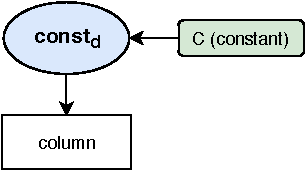
\includegraphics[width=0.8\linewidth]{expression_node-constant-decompression_2.pdf}
    \caption[b]{decompression}
    \label{fig:pd:constant:exprnode:decompression}
  \end{subfigure}
  \caption{Constant expression nodes}
  \label{fig:pd:constant:exprnode}
\end{figure}

The \textit{compression node} takes as input the constant column and does not generate any output column. Similarly, the \textit{decompression node} does not require any column to produce the constant column.

The compression and decompression operators are \(const_{c}\) and \(const_{d}\). The metadata they require is the constant \(C\). \(const_{c}\) takes as input a value \(v\) and checks whether it is equal to \(C\). If \textit{True}, then it returns nothing. Else, it raises an \textit{OperatorException} indicating that \(v\) is an exception and should be added to the exception column. \(const_{d}\) does not take any input value and returns the constant \(C\).

The benefit of the \nameref{subsec:pd:constant} representation scheme is clear: we avoid storing a column on disk. Dictionary encoding could also be used to compress constant columns, however it still stores a column with dictionary ids as opposed to no column at all. A more generic alternative representation for constant columns would be a \textit{whitebox} version of RLE that supports any data types.

% ---------------------------------------------------------------------------
% ----------------------- end of thesis sub-document ------------------------
% ---------------------------------------------------------------------------


\subsection{Numeric strings}
\label{subsec:pd:numericstrings}


% ----------------------- paths to graphics ------------------------

\graphicspath{{5_automatic_learning/pattern_detection/images/}}

% ----------------------- contents from here ------------------------
% 

This pattern detector searches for numbers stored in string columns. Once found, it changes the column data type to a numeric one, while also preserving the string format of the numbers in additional columns. The purpose is to optimize the data type and create opportunities for numeric compression schemes. The \textit{select\_column} method only returns \textit{True} for \verb|VARCHAR| columns. This is a single-column pattern detector and columns are evaluated independently. The next paragraphs describe the pattern detection process for a single column.

The \textit{scanning} phase checks for each value (\(v_{string}\)) whether it can be parsed as a number (\(v_{numeric}\)). If \textit{True}, it extracts the format information and checks whether the original string value can be reconstructed. The \textit{evaluation} phase chooses an appropriate numeric data type (e.g. \verb|DECIMAL(p,s)|) based on the type and range of the values selected in the \textit{scanning} phase. More details about the format preserving and data type inference processes are presented in the following paragraphs.

\textbf{Format preserving.} While analyzing the Public BI benchmark we noticed that the majority of string values \(v_{string}\) with a different format than their numeric representation \(v_{numeric}\) contain leading or trailing characters (e.g. zeros, whitespace). Therefore, we based our format preserving technique on 3 components---\textit{prefix}, \(v_{numeric}\), \textit{suffix}---as follows:\\
Step-1: cast \(v_{string}\) to number to obtain \(v_{numeric}\)\\
Step-2: check whether \(abs(v_{numeric})\) is a substring of \(v_{string}\). If \textit{False}, the format cannot be preserved. Otherwise, \(v_{string}\) has the following format:
\verb|${|\textit{prefix}\verb|}|\(abs(v_{numeric})\)\verb|${|\textit{suffix}\verb|}|,
where \textit{prefix} and \textit{suffix} can be any strings, including the empty string.\\
Step-3: extract the \textit{prefix} and \textit{suffix} and store them as format information together with \(v_{numeric}\).

\(v_{string}\) can be now reconstructed by concatenating the \textit{prefix}, \(v_{numeric}\) and \textit{suffix} values. Table~\ref{tab:pd:numericstring:formatexamples} illustrates a few examples that the format preserving technique covers (\verb|"_"| characters represent spaces).

\begin{table}[h]
\centering
\begin{tabular}{@{}llllll@{}}
\toprule
\(v_{string}\)    & \(v_{numeric}\) & \textit{prefix} & \(abs(v_{numeric})\) & \textit{suffix} & \textit{description}               \\ \midrule
\verb|"1.23"|     & \verb|1.23|     & \verb|""|       & \verb|1.23|          & \verb|""|       & no format information              \\
\verb|"1.2300"|   & \verb|1.23|     & \verb|""|       & \verb|1.23|          & \verb|"00"|     & trailing zeros                     \\
\verb|"000.1"|    & \verb|0.1|      & \verb|"00"|     & \verb|0.1|           & \verb|""|       & leading zeros                      \\
\verb|"+10"|      & \verb|10|       & \verb|"+"|      & \verb|10|            & \verb|""|       & \(+\) sign                         \\
\verb|"-10"|      & \verb|-10|      & \verb|"-"|      & \verb|10|            & \verb|""|       & negative number                    \\
\verb|"-000.5"|   & \verb|-0.5|     & \verb|"-00"|    & \verb|0.5|           & \verb|""|       & negative number with leading zeros \\
\verb|"__54\t\t"| & \verb|54|       & \verb|"__"|     & \verb|54|            & \verb|"\t\t"|   & leading and trailing whitespace    \\ \bottomrule
\end{tabular}
\caption{Numeric string format preserving examples}
\label{tab:pd:numericstring:formatexamples}
\end{table}

We do not support and consider exceptions the following: 1) numbers in scientific notation; 2) other notations or abbreviations (e.g. \verb|.12| instead of \verb|0.12|, \verb|1_000_000| instead of \verb|1000000|, etc.).

\textbf{Data type inference.} The purpose of this pattern detector is to store the numeric string values in a numeric column, which requires a numeric data type. We chose two data types that can be used to represent all numbers: \verb|DECIMAL(p,s)| and \verb|DOUBLE|. During the \textit{scanning} phase all \(v_{numeric}\) values are interpreted as decimals. The maximum number of digits before and after the decimal point---\(\mathit{integer}_{dmax}\) and \(\mathit{fractional}_{dmax}\)---are determined.  In the \textit{evaluation} phase, the parameters \textit{p} (precision) and \textit{s} (scale) of the \verb|DECIMAL(p,s)| data type are computed as follows:
\begin{equation}
\label{eq:pd:numericstrings:precisionscale}
\begin{array}{ll}
    p &= \mathit{integer}_{dmax} + \mathit{fractional}_{dmax}\\
    s &= \mathit{fractional}_{dmax}
\end{array}
\end{equation}
The final datatype of the numeric column is determined as follows:
\begin{equation}
\label{eq:pd:numericstrings:datatype}
\mathit{datatype} = 
\left\{
\begin{array}{ll}
    \verb|DECIMAL(p,s)| & \mbox{if } p \leq p_{max}\\
    \verb|DOUBLE| & \mbox{else}
\end{array}
\right.
\end{equation}
where:
\begin{itemize}
    \item[] \(p_{max}\) = maximum decimal precision supported by the system
\end{itemize}
The maximum precision value is configurable and necessary as database systems enforce it---MonetDB: \(p_{max}=38\) \cite{monetdbdatatypes}, VectorWise: \(p_{max}=39\) \cite{vectorwisedecimal}.

A string value \(v_{string}\) is considered an exception if any of the following conditions is not satisfied:\\
1) \(v_{string}\) cannot be parsed as a numeric value \(v_{numeric}\)\\
2) \(v_{string}\) cannot be reconstructed from its numeric value \(v_{numeric}\) and format information\\
3) \(v_{numeric}\) exceeds the numeric data type selected in the \textit{evaluation} phase

There is no strict filtering condition that determines whether a column fits this pattern or not. The pattern detector outputs a result for all columns with \textit{coverage} grater than \(0\), leaving the responsibility of choosing which columns to compress with this scheme to the compression learning algorithm. The \textit{evaluation result} is composed of the \textit{coverage} and \textit{row\_mask}---as defined in \ref{subsec:genericpd}~\nameref{subsec:genericpd}. No additional metadata is necessary for the compression and decompression processes.

The \textit{expression nodes} for the \nameref{subsec:pd:numericstrings} pattern are illustrated in the Figure~\ref{fig:pd:numericstrings:exprnode}.

\begin{figure}[h]
  \centering
  \begin{subfigure}[t]{0.49\linewidth}
    \centering
    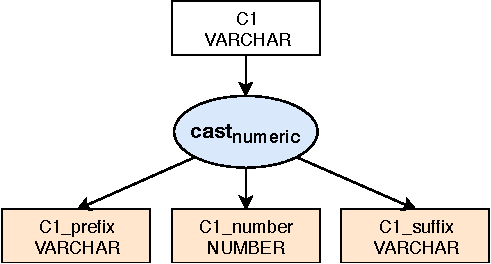
\includegraphics[width=1\linewidth]{expression_node-nas-compression_3.pdf}
    \caption[b]{compression}
    \label{fig:pd:numericstrings:exprnode:compression}
  \end{subfigure}
%   \hspace{1em}
  \begin{subfigure}[t]{0.49\linewidth}
    \centering
    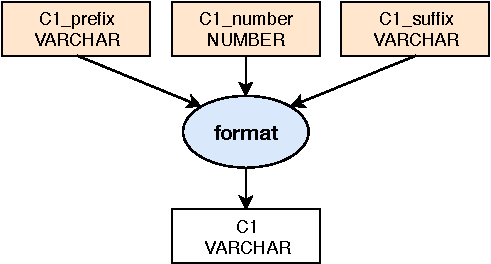
\includegraphics[width=1\linewidth]{expression_node-nas-decompression_3.pdf}
    \caption[b]{decompression}
    \label{fig:pd:numericstrings:exprnode:decompression}
  \end{subfigure}
  \caption{Numeric strings expression nodes}
  \label{fig:pd:numericstrings:exprnode}
\end{figure}

The \textit{compression node} takes as input the \textit{string} column and generates three output columns: one for storing the numeric values and the other two for storing the format information as \textit{prefix} and \textit{suffix}. The \textit{decompression node} takes as input the \textit{numeric}, \textit{prefix} and \textit{suffix} columns and reconstructs the original string column.

The compression operator \(cast_{numeric}\) takes as input \(v_{string}\) and tries to represent it as the 3 components---\textit{prefix}, \(v_{numeric}\) and \textit{suffix}---as described above. It then checks whether \(v_{numeric}\) fits in the inferred data type of the numeric column. If everything succeeds it returns the 3 values, else it raises an \textit{OperatorException} indicating that \(v_{string}\) should be added to the exception column. The decompression operator \(concat\) reconstructs \(v_{string}\) by concatenating \textit{prefix}, \(abs(v_{numeric})\) and \textit{suffix}. The two operators do not require any metadata, except for the numeric column data type.

There are two main benefits brought by this representation scheme: 1) using an optimal numeric data type instead of \verb|VARCHAR|, leading to smaller size on disk; 2) creating opportunities to further compress the numeric column with numeric compression schemes. Moreover, we noticed that in practice the \textit{prefix} and \textit{suffix} columns get further compressed as \nameref{subsec:pd:constant} or with \nameref{subsec:pd:dict} encoding.

% ---------------------------------------------------------------------------
% ----------------------- end of thesis sub-document ------------------------
% ---------------------------------------------------------------------------

\subsection{Character set split}
\label{subsec:pd:charsetsplit}


% ----------------------- paths to graphics ------------------------

\graphicspath{{5_automatic_learning/pattern_detection/images/}}

% ----------------------- contents from here ------------------------
% 

The \nameref{subsec:pd:charsetsplit} pattern detector searches for string columns where all values have the same structure in terms of character set sequences. A few examples are listed in Table~\ref{tab:pd:charsetsplit:examples} (\verb|"_"| characters represent spaces).

\begin{table}[h]
\centering
\begin{tabular}{@{}lll@{}}
\toprule
customer            & account             & transaction                 \\ \midrule
\verb|customer0001| & \verb|HHSI2452____| & \verb|{9AE2B97B-69D0-4A5E}| \\
\verb|customer0002| & \verb|TIRNO1017___| & \verb|{891F7B57-80C4-4BAA}| \\
\verb|customer0003| & \verb|TIRNO168823_| & \verb|{7C652BE6-947F-4AFF}| \\
\verb|...|          & \verb|...|          & \verb|...|                  \\
\verb|customer4735| & \verb|HHSI3391____| & \verb|{41AA2723-BA9D-465C}| \\
\verb|customer4736| & \verb|TIRNO41163__| & \verb|{88635130-6292-4C04}| \\ \bottomrule
\end{tabular}
\caption{Character set split examples}
\label{tab:pd:charsetsplit:examples}
\end{table}

The \textit{customer} column contains values that start with the constant \verb|customer| (charset: letters) and end with a number (charset: digits). All values on the \textit{account} column have the following structure: letters+digits+whitespace. The \textit{transaction} column contains 3 hex numbers (charset: hex digits) separated by dashes and enclosed in brackets (charset: delimiters).

The purpose of the \nameref{subsec:pd:charsetsplit} pattern detector is to split these columns into multiple columns based on the structure given by the character sets. For example, the \textit{customer} column is split into 2 columns: one containing the \verb|customer| constant value and one containing the numbers at the end. The \textit{transaction} column is split into 7 columns: 1 for the open bracket, 1 for the closed bracket, 2 for the dashes and 3 columns for the hex numbers.

The pattern detector receives two additional parameters: 1) \(coverage_{min}\)---used in the \textit{evaluation} phase to filter results; 2) a list of character sets (e.g. \verb|[a-zA-Z]|, \verb|[0-9a-fA-F]|, \verb|[_-{}()]|, etc.). The character sets can contain any characters, but they must be disjoint sets. An additional character set---the \textit{default} charset---is implicitly defined to represent all the other characters that are not in the sets provided as parameter. Multiple instances of this pattern detector can be used at the same time with different lists of character sets, leaving the learning algorithm to choose the one that provided the best results. This pattern detector works only with \verb|VARCHAR| columns. It is a single-column pattern detector and columns are evaluated independently. The next paragraphs describe the pattern detection process for a single column.

We define the \textit{get\_charset\_pattern} function as follows: \textit{input}: a string value (\(v_{s}\)) and a list of character sets (\(charset_{list}\)); \textit{output}: the \(charset_{pattern}\) of \(v_{s}\). The \(charset_{pattern}\) is a string that encodes the structure of \(v_{s}\) based on the provided \(charset_{list}\). The \textit{get\_charset\_pattern} function creates the \(charset_{pattern}\) by replacing groups of consecutive characters from the same charset with a placeholder. For example, a group of 3 digits will be replaced by the placeholder \verb|D|. The result of applying the \textit{get\_charset\_pattern} function on the columns in Table~\ref{tab:pd:charsetsplit:examples} is shown in Table~\ref{tab:pd:charsetsplit:charsetpattern} ("\verb|?|" is the default placeholder).

\begin{table}[h]
\centering
\begin{tabular}{l|lll}
\hline
column                & customer                      & account                      & transaction                 \\
\(charset_{list}\)    & \verb|[a-zA-Z]|, \verb|[0-9]| & \verb|[a-zA-Z]|,\verb|[0-9]| & \verb|[0-9a-fA-F]|          \\
placeholders          & \verb|L|, \verb|D|, \verb|?|  & \verb|L|, \verb|D|, \verb|?| & \verb|H|, \verb|?|          \\
\(v_{s}\)             & \verb|customer0001|           & \verb|HHSI2452____|          & \verb|{9AE2B97B-69D0-4A5E}| \\
\(charset_{pattern}\) & \verb|LD|                     & \verb|LD?|                   & \verb|?H?H?H?|              \\ \hline
\end{tabular}
\caption{Charset structure examples}
\label{tab:pd:charsetsplit:charsetpattern}
\end{table}

In the examples in Table~\ref{tab:pd:charsetsplit:examples} the values on each column give the same \(charset_{pattern}\) because they have the same structure. However, in practice this is not often the case. While analyzing the Public BI benchmark we distinguished the following cases, which depend both on the data values and the \(charset_{list}\):\\
1) no structure: many different \(charset_{pattern}\) values, with uniform distribution\\
2) fixed structure: a single \(charset_{pattern}\)\\
3) fixed structure with some exceptions: a single dominant \(charset_{pattern}\)\\
4) more than 1 fixed structure: a few (1-3) dominant \(charset_{pattern}\) values\\
Among these cases, we are interested in the last 3, the first one being filtered in the \textit{evaluation} phase.

The \textit{scanning} phase applies the \textit{get\_charset\_pattern} function to all values and builds the histogram of the resulting \(charset_{pattern}\) values. The \textit{evaluation} phase treats each \(charset_{pattern}\) as an independent result as follows: 1) computes the \textit{coverage} as the number of occurrences over the total number of non-null values; 2) computes the \textit{row\_mask} by marking the rows where the \(charset_{pattern}\) is present; 3) computes an additional evaluation metric: average percentage of chars that fit in one of the charsets (100\% - percentage of chars in the default charset). It then filters and returns the results that have a \(coverage\) greater than \(coverage_{min}\), leaving the learning algorithm to decide which result or combination of multiple results is the best. The metadata necessary for compression is composed of the \(charset_{list}\) and the \(charset_{pattern}\). The latter is different for each result. Decompression does not require any metadata.

The \textit{expression nodes} for the \nameref{subsec:pd:charsetsplit} pattern are illustrated in Figure~\ref{fig:pd:charsetsplit:exprnode}.

\begin{figure}[h]
  \centering
  \begin{subfigure}[t]{0.49\linewidth}
    \centering
    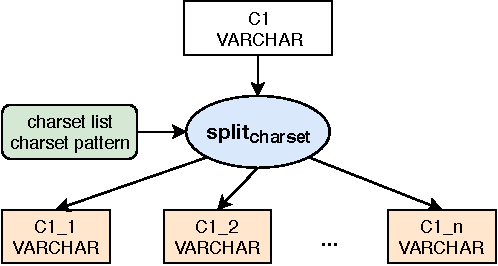
\includegraphics[width=1\linewidth]{expression_node-css-compression_2.pdf}
    \caption[b]{compression}
    \label{fig:pd:charsetsplit:exprnode:compression}
  \end{subfigure}
%   \hspace{1em}
  \begin{subfigure}[t]{0.49\linewidth}
    \centering
    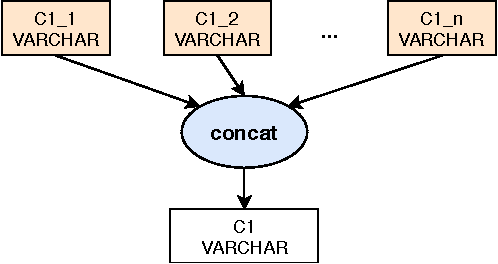
\includegraphics[width=1\linewidth]{expression_node-css-decompression_2.pdf}
    \caption[b]{decompression}
    \label{fig:pd:charsetsplit:exprnode:decompression}
  \end{subfigure}
  \caption{Character set split expression nodes}
  \label{fig:pd:charsetsplit:exprnode}
\end{figure}

The \textit{compression node} takes as input the string column and the compression metadata and outputs \(n\) \verb|VARCHAR| columns, where \(n = \mathit{len}(charset_{pattern})\)---one column for each character group. The \textit{decompression node} takes as input the \(n\) columns and concatenates them to reconstruct the original input column.

The compression operator \(split_{charset}\) takes as input the string value \(v_{s}\) and the compression metadata: \(charset_{list}\) and \(charset_{pattern}\). It applies the \textit{get\_charset\_pattern} function on \(v_{s}\) to obtain \(charset_{pattern}\_v\). It then compares \(charset_{pattern}\_v\) with \(charset_{pattern}\) to see if \(v_{s}\) has the correct structure. If they are not equal, it raises an \textit{OperatorException}, indicating that \(v_{s}\) is an exception. Otherwise, it splits \(v_{s}\) into \(n\) substrings---each one corresponding to a charset group---and returns them. The decompression operator \(concat\) receives as input \(n\) substrings and concatenates them to reconstruct the original value \(v_{s}\).

This representation scheme does not bring any compression benefit by itself. Instead, it creates compression opportunities by splitting columns into sub-columns that can be recursively compressed with other techniques. E.g. the columns in Table~\ref{tab:pd:charsetsplit:examples} can be compressed as follows:\\
1) the \textit{customer} column is first split into 2 columns: \textit{letters} and \textit{digits}. Then the \textit{letter} column is represented as a \nameref{subsec:pd:constant} and the \textit{digits} column is represented through a \nameref{subsec:pd:numericstrings} node and further compressed with numeric compression schemes (e.g. DELTA).\\
2) the \textit{account} column is split into 3 columns: \textit{letters}, \textit{digits}, \textit{spaces}. The \textit{letters} column gets compressed with \nameref{subsec:pd:dict} encoding. The \textit{digits} column is compressed similarly to the one in the \textit{customer} column. The \textit{spaces} column may be compressed through a custom representation scheme that identifies values with a single repeated character and only stores their number, or, alternatively, through \nameref{subsec:pd:dict} encoding, since the number of different space padding sequences is most likely small.\\
3) the \textit{transaction} column is split into 4 \textit{delimiter} columns and 3 \textit{hex} columns. All \textit{delimiter} columns have only 1 constant character and are compressed as \nameref{subsec:pd:constant}. The \textit{hex} columns can be represented through an implementation of \nameref{subsec:pd:numericstrings} that supports hexadecimal numbers, leading to 3 numeric columns that can benefit from numeric compression schemes.\\
In all three cases the \nameref{subsec:pd:charsetsplit} representation transforms an uncompressible \verb|VARCHAR| column into multiple compressed physical columns, significantly reducing the disk space required to store the data.

% ---------------------------------------------------------------------------
% ----------------------- end of thesis sub-document ------------------------
% ---------------------------------------------------------------------------

\subsection{Column correlation}
\label{subsec:pd:columncorrelation}


% ----------------------- paths to graphics ------------------------

\graphicspath{{5_automatic_learning/pattern_detection/images/}}

% ----------------------- contents from here ------------------------
% 

The purpose of the \nameref{subsec:pd:columncorrelation} pattern detector is to find correlations between columns and create mappings that can be used to represent a column as a function of another. The technique we describe is generic and can be applied to any data type. This pattern detector receives an additional parameter \(\mathit{corr\_coef}_{min}\), which indicates the minimum degree of correlation between two columns and is used to filter results in the \textit{evaluation} step. This is a multi-column pattern detector---it needs to analyze multiple columns at the same time.

\textbf{Correlation types.} From a statistical point of view, we can distinguish 3 types of correlations: between continuous, discrete and categorical variables. The first 2 apply to numeric values and can measure numerical similarities (e.g. sales increased as the marketing budget increased). The latter is less restrictive and works with any type of values. Categorical variables contain a finite number of values (e.g. payment method or customer satisfaction levels: low, high, very high, etc.) 
These can be further categorized into ordinal and nominal variables. Ordinal values have a natural ordering (e.g. tiny, small, large, huge) while nominal values have no ordering (e.g. names or colors).
TODO-1: references

While analyzing the Public BI benchmark we noticed that most correlations are between nominal values. Table~\ref{tab:pd:columncorrelation:nominalexample} shows a representative example from the \textit{CommonGovernment\_1} dataset.

\begin{table}[h]
\centering
\begin{tabular}{@{}ll@{}}
\toprule
short\_name  & ag\_name                                       \\ \midrule
\verb|GSA|   & \verb|GENERAL SERVICES ADMINISTRATION|         \\
\verb|GSA|   & \verb|GENERAL SERVICES ADMINISTRATION|         \\
\verb|HHS|   & \verb|DEPARTMENT OF HEALTH AND HUMAN SERVICES| \\
\verb|TREAS| & \verb|DEPARTMENT OF TREASURY|                  \\
\verb|TREAS| & \verb|DEPARTMENT OF TREASURY|                  \\
\verb|HHS|   & \verb|DEPARTMENT OF HEALTH AND HUMAN SERVICES| \\
\verb|GSA|   & \verb|GENERAL SERVICES ADMINISTRATION|         \\ \bottomrule
\end{tabular}
\caption{CommonGovernment\_1 nominal correlation}
\label{tab:pd:columncorrelation:nominalexample}
\end{table}


The table contains a name and its abbreviation repeated over multiple rows. The 2 columns are perfectly correlated because any value on one of the columns always has the same corresponding value on the other column (e.g. \verb|TREAS| on the \textit{short\_name} column always determines \verb|DEPARTMENT OF TREASURY| on the \textit{ag\_name} column).

Base on this observation, we decided to limit the scope of the \nameref{subsec:pd:columncorrelation} pattern detector to nominal categorical variables and interpret the values on all columns as nominal values. We leave the other correlation types as future work.

\textbf{Correlation coefficient \& mapping.} The \nameref{subsec:pd:columncorrelation} pattern detection process works in 3 phases: 1) compute the correlation coefficient (\(\mathit{corr\_coef}\)) for all pairs of 2 columns (\(c_{source}\), \(c_{target}\)); 2) select the pairs with \(\mathit{corr\_coef}\) higher than \(\mathit{corr\_coef}_{min}\); 3) create the correlation mapping (\(map_{obj}\)) that can be used to determine \(c_{target}\) based on \(c_{source}\).

The measure of association between 2 nominal categorical variables can be determined through existing statistical methods like Cramer's V \cite{cramir1946mathematical} or the Uncertainty coefficient Theil's U \cite{press1992theilsu}. Both methods are suitable for finding correlations between columns, but they only provide the measure of how well the columns are correlated as a number between 0 and 1---the correlation coefficient \(\mathit{corr\_coef}\). We still need the correlation mapping to be able to represent one column as a function of another.

We define the correlation mapping \(map_{obj}\) between 2 columns \(c_{source}\) and \(c_{target}\) as a dictionary with (\(v_{source}\), \(v_{target}\)) key-value pairs, where \(v_{source}\) are values from \(c_{source}\) and \(v_{target}\) are values from \(c_{target}\). Formally, the mapping is a total function \(f \colon S \to T\), where an element from T can be mapped to 0, 1 or multiple elements in S, as depicted in Figure~\ref{fig:pd:columncorrelation:totalfunction}.

\begin{figure}[h]
  \centering
  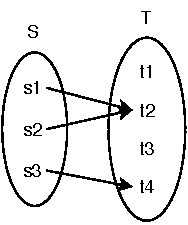
\includegraphics[width={0.23\linewidth}]{total_function_2.pdf}
  \caption{Mapping function}
  \label{fig:pd:columncorrelation:totalfunction}
\end{figure}

The process of creating the mapping between 2 columns \(c_{source}\) and \(c_{target}\) is depicted in Figure~\ref{fig:pd:columncorrelation:mapping}.

\begin{figure}[h]
  \centering
  \begin{subfigure}[t]{0.22\linewidth}
    \centering
    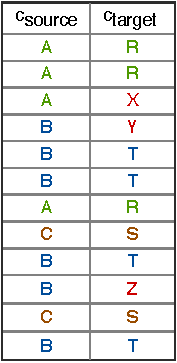
\includegraphics[width=1\linewidth]{mapping-corr-step_1_1.pdf}
    \caption[b]{Data values}
    \label{fig:pd:columncorrelation:mapping:step1}
  \end{subfigure}
  \hspace{3em}
  \begin{subfigure}[t]{0.23\linewidth}
    \centering
    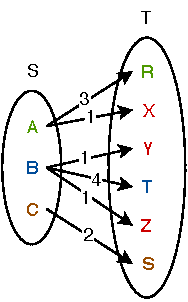
\includegraphics[width=1\linewidth]{mapping-corr-step_2_1.pdf}
    \caption[b]{Step-1}
    \label{fig:pd:columncorrelation:mapping:step2}
  \end{subfigure}
  \hspace{3em}
  \begin{subfigure}[t]{0.23\linewidth}
    \centering
    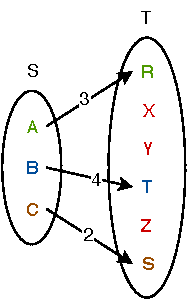
\includegraphics[width=1\linewidth]{mapping-corr-step_3_1.pdf}
    \caption[b]{Step-2}
    \label{fig:pd:columncorrelation:mapping:step3}
  \end{subfigure}
  \caption{Column correlation mapping}
  \label{fig:pd:columncorrelation:mapping}
\end{figure}

The correlation mapping is built in 2 steps. Step-1: for every unique value in \(c_{source}\) build the histogram of values in \(c_{target}\) it is associated with. In the example in Figure~\ref{fig:pd:columncorrelation:mapping}, \verb|B| is associated with \verb|T| 4 times and with \verb|Y| and \verb|Z| one time. Step-2: for every unique value in \(c_{source}\) select the value in \(c_{target}\) it is associated with the most (i.e. the one with the highest number of occurrences). In the example, \verb|R| is to most common value for \verb|A|, \verb|T| is the most common value for \verb|B| and \verb|S| is the only value associated with \verb|C|. These selected pairs of values form the correlation mapping \(map_{obj}\).

We consider exceptions all the values from \(c_{target}\) that are not present in \(map_{obj}\). The \(exception\_ratio\) is given by the total number of values on \(c_{target}\) that do not respect the correlation mapping.

We observe that two columns that have \(exception\_ratio = 0\) are perfectly correlated (i.e. all values in \(c_{target}\) can be determined from \(c_{source}\)). Conversely, two columns with \(exception\_ratio = 1\) are completely uncorrelated. We can define, then, an alternative correlation coefficient: 
\(\mathit{corr\_coef} = 1 - exception\_ratio\). We compared it with existing methods (Cramer's V and Theil's U) by computing the correlation coefficient for tables in the Public BI benchmark. We analyzed the results and concluded that all three methods are similar and correctly identify correlations between nominal columns. The advantage of our approach is that it also gives the correlation mapping---which we are interested in---without any time complexity overhead: \(\mathcal{O}(n)\), where \(n\) is the total number of values in the sample. For this reason, we decided to used it in our implementation instead of Cramer's V or Theil's U.

In terms of the pattern detection process, the histograms are built in the \textit{scanning} phase and the correlation coefficient and mapping are computed in the \textit{evaluation} phase. The compression and decompression metadata resulted from this process is the correlation map \(map_{obj}\). The pattern detector outputs all (\(c_{source}, c_{target}\)) pairs with \(\mathit{corr\_coef} > \mathit{corr\_coef}_{min}\), leaving the task of choosing between the results to the learning algorithm. The \textit{evaluation result} is composed of the \textit{coverage} and \textit{row\_mask}---as defined in \ref{subsec:genericpd}~\nameref{subsec:genericpd}---and the correlation coefficient.

The \textit{expression nodes} for the \nameref{subsec:pd:columncorrelation} pattern are illustrated in Figure~\ref{fig:pd:columncorrelation:exprnode}.

\begin{figure}[h]
  \centering
  \begin{subfigure}[t]{0.45\linewidth}
    \centering
    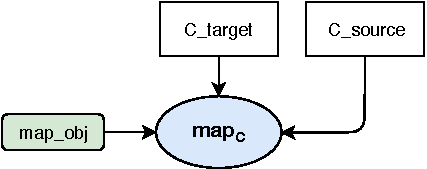
\includegraphics[width=1\linewidth]{expression_node-corr-compression_3.pdf}
    \caption[b]{compression}
    \label{fig:pd:columncorrelation:exprnode:compression}
  \end{subfigure}
  \hspace{3em}
  \begin{subfigure}[t]{0.30\linewidth}
    \centering
    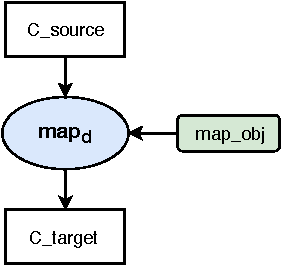
\includegraphics[width=1\linewidth]{expression_node-corr-decompression_3.pdf}
    \caption[b]{decompression}
    \label{fig:pd:columncorrelation:exprnode:decompression}
  \end{subfigure}
  \caption{Column correlation expression nodes}
  \label{fig:pd:columncorrelation:exprnode}
\end{figure}

The \textit{compression node} takes as input the target column (\(c_{target}\)), the source column (\(c_{source}\)) and the metadata (\(map_{obj}\)). It does not generate any output column. The \textit{decompression node} takes as input \(c_{source}\) and \(map_{obj}\) and reconstructs \(c_{target}\) based on the mapping.

The compression operator \(map_{c}\) takes as input a target value (\(v_{target}\)), a source value (\(v_{source}\)) and the metadata (\(map_{obj}\)) and checks whether the key-value pair (\(v_{source}\), \(v_{target}\)) is present in \(map_{obj}\). If True, then it does nothing---\(v_{target}\) can be reconstructed based on \(v_{source}\). Otherwise, it raises an \textit{OperatorException} indicating that \(v_{target}\) cannot be retrieved from the mapping and needs to be stored in the exception column. The decompression operator \(map_{d}\) takes as input \(v_{source}\) and \(map_{obj}\) and returns the value from \(map_{obj}\) associated to \(v_{source}\): \(map_{obj}[v_{source}] = v_{target}\).

The benefit of the \nameref{subsec:pd:columncorrelation} compression scheme is clear: we avoid storing a column by representing it as a function of another column. However, this comes at the cost of storing the mapping between the 2 columns. Thus, it is only worth using this method when the mapping is small. The mapping size is dependent on the cardinality of the sets of values in the 2 columns. This is similar to \nameref{subsec:pd:dict} encoding and therefore we can state that \nameref{subsec:pd:columncorrelation} is effective only when both source and target columns are dictionary compressible.  With this new constraint, we can limit the scope of the \nameref{subsec:pd:columncorrelation} pattern detector to output columns of \textit{whitebox} \nameref{subsec:pd:dict} nodes, leading to the following benefits: 1) reduced detection time---less column pairs that need to be checked; 2) reduced mapping size---dictionary ids instead of string values. Due to the generic nature of \textit{whitebox} compression, this constraint can be implicitly satisfied by just adding a rule to the \textit{select\_column} method of the \nameref{subsec:pd:columncorrelation} pattern detector and letting the learning algorithm perform the recursive compression.

% ---------------------------------------------------------------------------
% ----------------------- end of thesis sub-document ------------------------
% ---------------------------------------------------------------------------


\subsection{Dictionary}
\label{subsec:pd:dict}


% ----------------------- paths to graphics ------------------------

\graphicspath{{5_automatic_learning/pattern_detection/images/}}

% ----------------------- contents from here ------------------------
% 

We implemented a \textit{whitebox} version of Dictionary encoding to serve as a prior compression step before \nameref{subsec:pd:columncorrelation}. The pattern detector receives an additional parameter \(size_{max}\)---maximum size of the dictionary. We restricted its scope to \verb|VARCHAR| columns. This is a single-column pattern detector and columns are evaluated independently. The next paragraphs describe the pattern detection process for a single column.

Dictionary encoding only produces good results on columns that have a small number of unique values. However, it is hard to reliably quantify this property when analyzing only a sample of the data. Moreover, the distribution of unique values may be skewed, with only a few values with high frequency and a long tail of low frequency values. For the purpose of our pattern detector, we addressed this issue by enforcing a maximum dictionary size (in bytes) and only keeping the most common values in the dictionary. This approach is also suitable if blocks of data are compressed independently: dictionaries need to be small as they are assigned per block. There are other (possibly better) ways of optimizing the dictionary values and size. However, this is not a core aspect for our pattern detector, since we only use it as an intermediate step required for \nameref{subsec:pd:columncorrelation}.

The dictionary is built as follows. The \textit{scanning} phase creates the histogram of all the values in the sample. In the \textit{evaluation} step we select as many values (\(v_{s}\)) from the histogram---in decreasing order of their number of occurrences---such that their total size is smaller or equal to the maximum size of the dictionary (\(size_{max}\)). The dictionary is represented as an array containing the selected values. The indices in the array represent the dictionary ids (\(v_{id}\)) used to encode the values (\(v_{s}\)). The dictionary represents the compression and decompression metadata. All the values that are not present in the dictionary are considered exceptions.

The pattern detector only outputs results for columns that are dictionary compressible. This decision is taken based on the estimated size of the input column, output columns and metadata:
\begin{equation}
\label{eq:pd:dict:outputcondition}
    size_{in} > size_{out} + size_{ex} + size_{metadata}
\end{equation}
where:
\begin{itemize}
    \item[] \(size_{in}\) = estimated size of the input column
    \item[] \(size_{out}\) = estimated size of the dictionary ids column
    \item[] \(size_{ex}\) = estimated size of the exceptions column
    \item[] \(size_{metadata}\) = size of the dictionary
\end{itemize}

If the above condition is \textit{True}, the input column is considered dictionary compressible and the pattern detector outputs a result for it. More details about how these sizes are computed are given in \ref{subsub:estimator:dict}~\nameref{subsub:estimator:dict}. The \textit{evaluation result} is composed of the \textit{coverage} and \textit{row\_mask}---as defined in \ref{subsec:genericpd}~\nameref{subsec:genericpd}.

The \textit{expression nodes} for the \nameref{subsec:pd:dict} pattern are illustrated in Figure~\ref{fig:pd:dict:exprnode}.

\begin{figure}[h]
  \centering
  \begin{subfigure}[t]{0.4\linewidth}
    \centering
    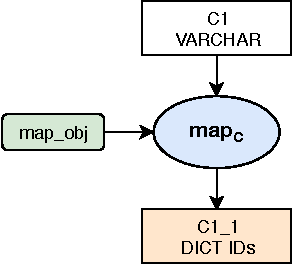
\includegraphics[width=0.8\linewidth]{expression_node-dictionary-compression_3.pdf}
    \caption[b]{compression}
    \label{fig:pd:dict:exprnode:compression}
  \end{subfigure}
  \hspace{1em}
  \begin{subfigure}[t]{0.4\linewidth}
    \centering
    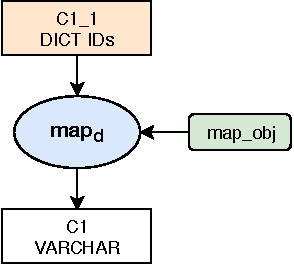
\includegraphics[width=0.8\linewidth]{expression_node-dictionary-decompression_3.pdf}
    \caption[b]{decompression}
    \label{fig:pd:dict:exprnode:decompression}
  \end{subfigure}
  \caption{Dictionary expression nodes}
  \label{fig:pd:dict:exprnode}
\end{figure}

The \textit{compression node} takes as input the string column and the dictionary \(map\_obj\). It outputs a column containing dictionary ids. The \textit{decompression node} takes as input the dictionary ids column and the dictionary and reconstructs the original input column.

The compression operator \(map_{c}\) takes as input the string value \(v_{s}\) and the dictionary \(map\_obj\) and outputs a dictionary id: the index of \(v_{s}\) in the array \(map\_obj\). As an optimization for the compression phase, \(map\_obj\) is represented as an actual dictionary with (\(v_{s}\), \(\mathit{index\_of}(v_{s})\)) key-value pairs instead of an array. If \(v_{s}\) is not found in \(map\_obj\) an \textit{OperatorException} is raised, indicating that \(v_{s}\) is an exception and should be stored in the exception column. The decompression operator \(map_{d}\) takes as input a dictionary id \(v_{id}\) (i.e. an index in the \(map\_obj\) array) and returns the original value \(v_{s}\) (\(map\_obj[v_{id}]\)).

% ---------------------------------------------------------------------------
% ----------------------- end of thesis sub-document ------------------------
% ---------------------------------------------------------------------------

% \subsection{n-gram frequency split}
\label{subsec:pd:ngramfreqsplit}


% ----------------------- paths to graphics ------------------------



% ----------------------- contents from here ------------------------
% 

\begin{verbatim}
TODO
\end{verbatim}

\iffalse
* general description of what it does
* additional parameters
* select\_column
* single/multi column

* pattern detection process
  - scanning
  - evaluation
  - metadata

* condition for outputting a result
* exception
* evaluation result

* expression node
  - I/O description
  - image

* operator (compression \& decompression):
  - metadata
  - functionality

* further compression opportunities
\fi

% ---------------------------------------------------------------------------
% ----------------------- end of thesis sub-document ------------------------
% ---------------------------------------------------------------------------

\iffalse
* general description of what it does
* additional parameters
* select\_column
* single/multi column

* pattern detection process
  - scanning
  - evaluation
  - metadata

* condition for outputting a result
* exception
* evaluation result

* expression node
  - I/O description
  - image

* operator (compression \& decompression):
  - metadata
  - functionality

* further compression opportunities
\fi

\iffalse
\begin{equation}
\label{eq:optimizationproblem:b}
    b = \mathit{avg}(c_{out})
\end{equation}
where:
\begin{itemize}
    \item[] \(n\) = total number of expression nodes
    \item[] \(c_{in}\) = number of input columns
\end{itemize}
\fi

% ---------------------------------------------------------------------------
% ----------------------- end of thesis sub-document ------------------------
% ---------------------------------------------------------------------------